\documentclass[11pt,a4paper]{article}
\usepackage[margin=2.5cm]{geometry}
\usepackage{graphicx}
\usepackage{enumitem}
\usepackage[svgnames]{xcolor}
\usepackage[most]{tcolorbox}
\usepackage[hidelinks]{hyperref} % o usar colorlinks como se explicó antes
\usepackage{listings}
\usepackage[spanish]{babel}
\usepackage{changepage}
\usepackage{enumitem}
\usepackage{capt-of}

\lstset{
	language=C, % Lenguaje: C
	basicstyle=\ttfamily\small, % Fuente monoespaciada, tamaño pequeño
	keywordstyle=\color{Blue}\bfseries, % Palabras clave en azul y negrita
	stringstyle=\color{Red}, % Cadenas en rojo
	commentstyle=\color{Green}, % Comentarios en verde
	numbers=left, % Numeración de líneas a la izquierda
	numberstyle=\tiny\color{Gray}, % Estilo de números de línea
	stepnumber=1, % Numerar cada línea
	numbersep=5pt, % Distancia de números al código
	showspaces=false, % No mostrar espacios
	showstringspaces=false, % No marcar espacios en cadenas
	frame=single, % Marco alrededor del código
	tabsize=4, % Tamaño de tabulación
	breaklines=true, % Romper líneas largas
	breakatwhitespace=true, % Romper solo en espacios
}

\begin{document}
	\begin{titlepage}
		\begin{center}
			\begin{figure}
				\centering
				
\includegraphics[scale=0.2]{US-marca-principal.png}
			\end{figure}
			{\large \textbf{Escuela Técnica Superior de Ingeniería Informática}}
			\vspace{2mm}\\
			{Ingeniería Informática. Ingeniería de Computadores.}
			\vspace{60mm}\\
			\begin{center}
				{\huge \textbf{MEMORIA PRÁCTICA \uppercase\expandafter{\romannumeral 2\relax}}}\\[2mm]
				{Asignatura: Sistemas Empotrados y de Tiempo Real I}\\
				{Profesor: Gabriel Jiménez Moreno}
			\end{center}
			\vfill
			{Alumno: Álvaro José Gullón Vega}
		\end{center}
	\end{titlepage}
	\pagebreak
	\tableofcontents
	\pagebreak
	
	\section{Objetivos}
	\large{
		En esta segunda práctica distinguimos dos objetivos:
		
		\subsection{Académico}
		Los objetivo académicos en este caso, constan de estudiar y entender el funcionamiento de los Displays LCD tradicionales que se usan con los microcontroladores, conocer los aspectos más básicos de la placa de desarrollo de la asignatura y entender las diferencias entre las diversas librerías que proporcionan los fabricantes para el manejo de los periféricos en los microcontroladores tipo Cortex.
		
		\subsection{Práctico}
		Para conseguir estos objetivos académicos, se han propuestos estos objetivos prácticos:
		\begin{itemize}
		\item Mandar texto a cualquier posición en un display tipo HD44780.
		\item Definir un nuevo dibujo en la memoria del Display y visualizarlo en pantalla
		\item Manejar los LEDs y el botón de la placa al igual que se hizo en la práctica 1.
		correspondientes a ese pin y conectadas a VCC o a GND.
		\item Sustituir en la librería del display LCD, que se proporciona en esta práctica, las llamadas a las funciones GPIO LL por funciones equivalentes GPIO HAL.
		\end{itemize}
	}
	
	\section{Introducción}
	\large{
		Como hemos mencionado en los objetivos, esta segunda práctica nos acercará a conocer los Display LCD al igual que nos ofrecerá una primera toma de contacto con la placa que usaremos en la asignatura.\\
		
		Las interfaces visuales más primitivas están basadas en LEDs, un ejemplo de ellos los displays de siete segmentos, los que si agrupamos varios de ellos podemos componer una interfaz visual más completa con un problema que es la cantidad de pines que se requieren para su control. Por otra parte contamos con los displays LCD u OLED, dos tecnologías que han evolucionado mucho los últimos años con las que se construyen un gran número de dispositivos de visualización destinados a su uso con microcontroladores.
		
		Nosotros, en SETR1, nos vamos a centrar en el uso de displays más modestos y primitivos que suelen disponer de dos tipos de interfaces:
		\begin{itemize}
			\item \textbf{Paralela:} Consiste en un bus de ocho bits \textit{(D0-D7)} y tres líneas de control \textit{(RS, E, R/W)}. El bus de datos es bidireccional de forma que podemos escribir en el display o podemos leer de él como por el ejemplo el bit de estado.
			
			\begin{center}
				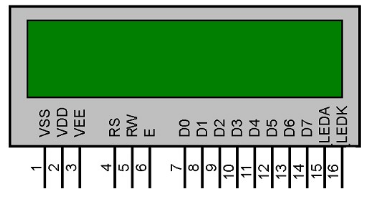
\includegraphics[width=0.6\textwidth]{pinout-display.png}
				\captionof{figure}{Pinout típico del Display LCD.}
			\end{center}
			
			\item \textbf{Serie síncrona:} Usan normalmente puertos \textit{I2C} o \textit{SPI}. Se utilizan dos o tres líneas de conexión con el microcontrolador.
		\end{itemize}
		
		El circuito de control es el cerebro del display, por un lado tiene los pines que sirven de interfaz con el usuario y por otra controla la pantalla de visualización. Casi siempre suelen tener una memoria RAM, excepto los más sofisticados que incluyen de dos en adelante para por ejemplo en la GameBoy organizarlas como memoria principal, memoria de background, memoria de tejas, etc...\\
		
		La pantalla donde se muestra la información en ocasiones su tamaño es independiente de la capacidad de direccionamiento de la memoria del controlador, y no tienen por qué coincidir. Otro aspecto a tener en cuenta es la resolución de cada carácter, el nuestro tiene 5 columnas por 8 filas de pixel, con 2x16 caracteres y con una anchura total de 6,5 cm.\\
		
		Para usar el HD44780 se realiza una conexión pin a pin con los GPIO del microcontrolador. Se suele colocar un potenciómetro que lo hace es regular en contraste de la pantalla. Para transferir datos, podemos usar \textit{D0-D7} o \textit{D4-D7}, en este último caso necesitamos dos accesos, primero 4 bits y después los otros 4 bits restantes. La librería software que vamos a usar en esta práctica para el manejo del HD44780 utiliza la interfaz de 4 bits y
		esperas entre transferencias, sin preguntar por el estado del dispositivo (si está Busy), y por tanto sin utilizar la línea
		R/W, sólo se hacen escrituras al LCD. Hay muchas librerías en internet para estos LCD y para múltiples plataformas
		y microcontroladores, ésta que vamos a usar es una de tantas, sin ninguna característica especial.\\
		
		El software para usar el display HD44780 es muy simple, primero hay una fase de inicialización (función \textit{lcd\_reset()} + función \textit{lcd\_display\_settings(1,0,0}) en la que se configura una serie de características, las más importante son si se va a usar el bus de conexión completo o sólo la parte alta (D0-D7 ó D4-D7) y si la pantalla es de una o dos
		líneas. En nuestro caso sabremos si la inicialización ha ido bien cuando observemos que se “ven” activas las dos líneas de la pantalla, y no sólo una.\\
		
		En el HD44780 se pueden hacer las siguientes operaciones:
		\begin{itemize}
			\item \textbf{Escritura (función lcd\_write(byte, rs):} se transfiere un byte y se indica si es un dato a la memoria o un comando (parámetro rs).
			
			\item \textbf{Apuntar CGRAM (lcd\_cgram\_address(uint8\_t address)):} cuando se usa esta función se manda un comando que sitúa el puntero de dirección en la CGRAM y apuntando a una determinada dirección.
			
			\item \textbf{Apuntar a la DDRAM (lcd\_display\_address(uint8\_t address)):} si queremos que vuelvan a visualizarse los datos en la pantalla tenemos que hacer que el apuntador vuelva a apuntar a una dirección de la DDRAM.
			
			\item \textbf{moveToXY(unsigned char row, unsigned char column):} con ella situamos el
			cursor en la fila/columna de la pantalla que queramos, como es natural hay que usar esa función primero y después mandar el texto que se quiera ver en la pantalla.
			
			\item \textbf{lcd\_print(char string[]):} sirve para visualizar una cadena de caracteres.
			
			\item \textbf{writeIntegerToLCD(int integer): se utiliza para mostar un entero.} 
			
			\item \textbf{lcd\_clock():} es la encargada de subir y bajar la línea de habilitación E.

			\item \textbf{lcd\_clear():} nos permite limpiar el contenido de la pantalla de nuestro display.\\
		\end{itemize}
		
		En microcontroladores complejos, como los ARM Cortex, el uso de librerías es esencial para desarrollar rápidamente. Aunque el núcleo ARM está estandarizado por la empresa ARM, los periféricos y el hardware adicional varían según el fabricante. ARM proporciona una interfaz estándar llamada CMSIS, útil pero limitada, ya que no incluye funciones prácticas para manejar el hardware específico de cada fabricante.\\
		
		Para facilitar el desarrollo, cada fabricante ofrece sus propias librerías. Por ejemplo, STMicroelectronics proporciona dos:
				\begin{itemize}
			\item \textbf{HAL (Hardware Abstraction Layer):} de alto nivel, fáciles de usar y portables, aunque menos eficientes.
			
			\item \textbf{LL (Low Layer):} de bajo nivel, más cercanas al hardware, optimizadas y potentes, pero más complejas.\\
		\end{itemize}
		
		Las HAL intentan ser universales dentro de cada fabricante y son comúnmente utilizadas por principiantes. En cambio, las LL ofrecen mayor control y rendimiento, ideales para desarrolladores con más experiencia. En esta práctica se estudiarán ambas aplicadas a los periféricos GPIO.\\
		
		Los pines GPIO se agrupan en puertos de 16 bits (GPIOA, GPIOB, etc.). Cada pin se identifica por su puerto y número (por ejemplo, PA1 o PC2). Para manipular estos pines se utilizan registros de 32 bits y funciones específicas. Así, tenemos el siguiente grupo de funciones LL para manejar los GPIO:
		\begin{lstlisting}
		LL_GPIO_IsOutputPinSet(GPIO_TypeDef *GPIOx, uint32_t PinMask) // lee uno o varios pines de un
		puerto de salida
		LL_GPIO_IsInputPinSet(GPIO_TypeDef *GPIOx, uint32_t PinMask) // lee uno o varios pines de un
		puerto de entrada
		LL_GPIO_SetOutputPin(GPIO_TypeDef *GPIOx, uint32_t PinMask) // pone a uno pin/pines
		LL_GPIO_ResetOutputPin(GPIO_TypeDef *GPIOx, uint32_t PinMask) // pone a cero pin/pines
		LL_GPIO_TogglePin(GPIO_TypeDef *GPIOx, uint32_t PinMask) // complementa pin/pines
		\end{lstlisting}
		
		\begin{lstlisting}
		LL_GPIO_ReadOutputPort(GPIO_TypeDef *GPIOx) // lee un puerto de salida entero
		LL_GPIO_WriteOutputPort(GPIO_TypeDef *GPIOx, uint32_t PortValue) // escribe un puerto entero
		\end{lstlisting}
		\vspace{1em}
		
		Por último, vamos a tratar con la placa \textbf{B-L475E-IOT01A} con el microcontrolador \textbf{STM32L475}:
		\begin{center}
			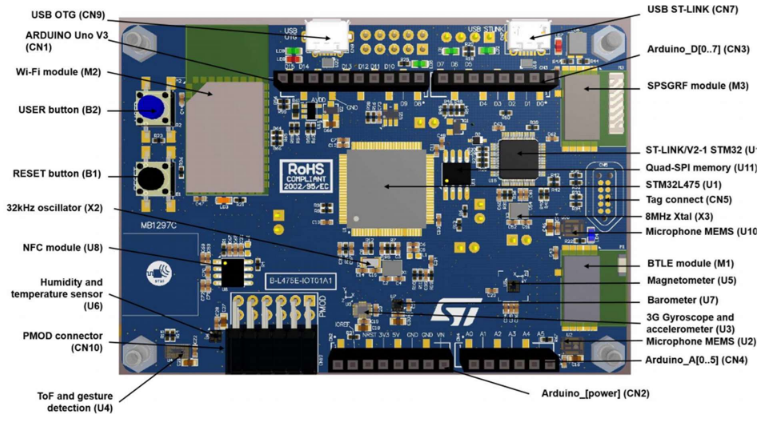
\includegraphics[width=0.6\textwidth]{bl475.png}
			\captionof{figure}{Placa \textbf{B-L475E-IOT01A} y elementos que la componen.}
		\end{center}
		
		Los aspectos más destacables de esta placa que nos conviene conocer es que el depurador ST-LINK vía USB sobre la misma placa que nos permite tres tipos de dispostivos: depurador, unidad de almacenamiento ficticio "masiva" y puerto virtual COM. También contiene un conector tipo Arduino.
	}
	
	\section{Desarrollo de la práctica}
	\subsection{Fase 1: Usar el display HD44780 y empezar a manejar la placa de la asignatura.}
	Lo primero que haremos será colocar el shield del display sobre la placa, teniendo en cuenta la orientación de esta para que los pines vayan en su sitio, para que sea más fácil, podemos retirar el "embellecedor" del botón azul para que no haga de escalón y no esté la placa puesta de aquella manera. Una vez colocada, conectaremos la placa a nuestro equipo usando el USB y conectándolo a la entrada \textit{USB ST-LINK} y procederemos a crear un nuevo proyecto y cuando nos salga la ventana de \textit{Target Selection} seleccionamos \textit{Board Selector} y buscamos nuestra placa, colocamos el nombre de nuestro proyecto y cuando nos pregunte si queremos inicializar los periféricos diremos que sí. Cuando se cree, se llevará un proceso que puede tardar bastante pues se está descargando las librerías del generador de código.
	
	\subsection{Fase 2: Repetir la Fase 2 y 4 de la práctica 1 con la nueva placa.}
	
	\subsection{Fase 3: Repetir la fase 1 de esta práctica, pero usando librerías HAL.}

	\section{Contestación de preguntas}
	
	\section{Conclusiones}

\end{document}